\documentclass{article}
\usepackage{graphicx} % Required for inserting images
\usepackage{float}
\usepackage[T1]{fontenc}
\usepackage{amsmath}
\usepackage[margin=1in]{geometry}
\usepackage{booktabs}
\usepackage{tabularx}
\usepackage[hidelinks]{hyperref}

\title{A minimum-variance (vega-adjusted) hedge on the stress-sized SPY put book}
\author{Experiment report \textperiodcentered{} L/S Gamma Desk, QUANTT}
\date{2026-11-02}

\begin{document}

\maketitle

\textbf{Question:} On the 35\% stress-sized \texttt{hedged} put book, does hedging each put to its delta plus a Hull-White-style vega term make the daily tail and the maximum drawdown less severe, without costing more than \$5,000 of net P\&L?

\textbf{Method:}

\begin{itemize}

\item \textbf{Pre-registration.} The hypothesis card was committed before any run (commit 3ab834b).

\item \textbf{Data and book.} The 2026-10-22 \texttt{hedged} book is replayed on R2 replay snapshots v1 (config\_hash b040760187f0) over the development window 2014-06-02 to 2024-12-31. The hold-out (2025-01-01 to 2026-07-10) was not used.

\begin{itemize}

\item The book is an always-on short 25-delta put, sized at entry to a 35\% stress budget: a one-day 20\% drop with IV at max(60\%, the put's IV) may cost at most \$87,500.

\item It is hedged daily at 10:15 with a 10-share band. The 1x-credit stop, 50\% profit-take and 7-DTE exit apply; the stop and the profit-take measure the put's P\&L including its hedge, as in the live rules.

\end{itemize}

\item \textbf{New switch.} Research-only \texttt{[backtest] mv\_\allowbreak{}hedge = k}. Each put's hedge target becomes its delta target plus k \ensuremath{\times} vega \ensuremath{\times} \ensuremath{\beta} /\allowbreak{} S per share of exposure.

\begin{itemize}

\item \ensuremath{\beta} is the slope of daily VIX-point changes on SPY daily returns over the trailing 252 completed days, refit each day.

\item For a short put \ensuremath{\beta} is negative, so the hedge sells more shares than the delta alone. Sizing is unchanged.

\end{itemize}

\item \textbf{Variants:} \texttt{mv} = k 1 (primary); \texttt{mv\_\allowbreak{}half} = k 0.5.

\item \textbf{Reference.} The registered \texttt{2026-\allowbreak{}10-\allowbreak{}22-\allowbreak{}stress-\allowbreak{}sized-\allowbreak{}puts/\allowbreak{}hedged} runs, reused and not rerun, at the same spread multiple.

\item \textbf{Runs and costs.} Every variant was run at 1x and 2x spreads. Costs are \$0.65 per contract and \$0.005 per share, with a \$1 minimum per order. Decisions, exits and hedges run at 10:15 ET.

\end{itemize}

\section{Result vs the pass bar}

Every check had to hold at 1x and 2x. P\&L is net of spreads and commissions, in USD, for the sized book. ES 5\% is the mean of the worst 5\% of daily net P\&L.

\begin{center}\small
\begin{tabularx}{\linewidth}{>{\raggedright\arraybackslash}X l >{\raggedright\arraybackslash}X l >{\raggedright\arraybackslash}X l}
\toprule
\textbf{Check (\texttt{mv} vs \texttt{hedged})} & \textbf{1x value} & \textbf{1x bar} & \textbf{2x value} & \textbf{2x bar} & \textbf{Result} \\
\midrule
ES 5\%, full window & \ensuremath{-}\$2,828 & less severe than \ensuremath{-}\$3,016 & \ensuremath{-}\$2,871 & less severe than \ensuremath{-}\$3,094 & pass \\
Max drawdown, full window & \$41,112 & < \$70,362 & \$41,119 & < \$75,488 & pass \\
Net P\&L, full window & \$104,049 & \ensuremath{\geq} \$116,482 & \$79,425 & \ensuremath{\geq} \$96,172 & fail \\
Round trips (floor \ensuremath{\geq} 30, 1x) & 193 &  &  &  & met \\
\bottomrule
\end{tabularx}
\end{center}

\textbf{Verdict: failed.} The vega-adjusted hedge cut the tail and the drawdown, but it made \$17.4k less than the delta hedge at 1x and \$21.7k less at 2x, more than the \$5k allowed. The book still makes money: +\$104k at 1x and +\$79k at 2x.

\subsection{Full-window numbers (not part of the bar)}

\begin{center}\small
\begin{tabularx}{\linewidth}{>{\raggedright\arraybackslash}X >{\raggedright\arraybackslash}X >{\raggedright\arraybackslash}X >{\raggedright\arraybackslash}X >{\raggedright\arraybackslash}X >{\raggedright\arraybackslash}X >{\raggedright\arraybackslash}X}
\toprule
\textbf{} & \textbf{\texttt{hedged} 1x} & \textbf{\texttt{mv} 1x} & \textbf{\texttt{mv\_\allowbreak{}half} 1x} & \textbf{\texttt{hedged} 2x} & \textbf{\texttt{mv} 2x} & \textbf{\texttt{mv\_\allowbreak{}half} 2x} \\
\midrule
Net P\&L & \$121,482 & \$104,049 & \$55,966 & \$101,172 & \$79,425 & \$29,367 \\
Net P\&L, 2014-06 to 2019-12 & \$49,132 & \$15,781 & \$24,217 & \$42,687 & \$7,233 & \$13,980 \\
Net P\&L, 2020-01 to 2024-12 & \$72,350 & \$88,268 & \$31,749 & \$58,485 & \$72,191 & \$15,387 \\
Sharpe & 0.52 & 0.42 & 0.29 & 0.43 & 0.33 & 0.15 \\
Max drawdown & \$70,362 & \$41,112 & \$44,012 & \$75,488 & \$41,119 & \$54,028 \\
ES 5\% (daily) & \ensuremath{-}\$3,016 & \ensuremath{-}\$2,828 & \ensuremath{-}\$2,678 & \ensuremath{-}\$3,094 & \ensuremath{-}\$2,871 & \ensuremath{-}\$2,800 \\
Round trips & 182 & 193 & 179 & 181 & 192 & 179 \\
Commissions (options /\allowbreak{} hedges) & \$5,955 /\allowbreak{} \$2,868 & \$6,448 /\allowbreak{} \$3,138 & \$5,802 /\allowbreak{} \$2,996 & \$5,918 /\allowbreak{} \$2,863 & \$6,400 /\allowbreak{} \$3,137 & \$5,802 /\allowbreak{} \$2,995 \\
\bottomrule
\end{tabularx}
\end{center}

\section{Charts}

\begin{figure}[H]\centering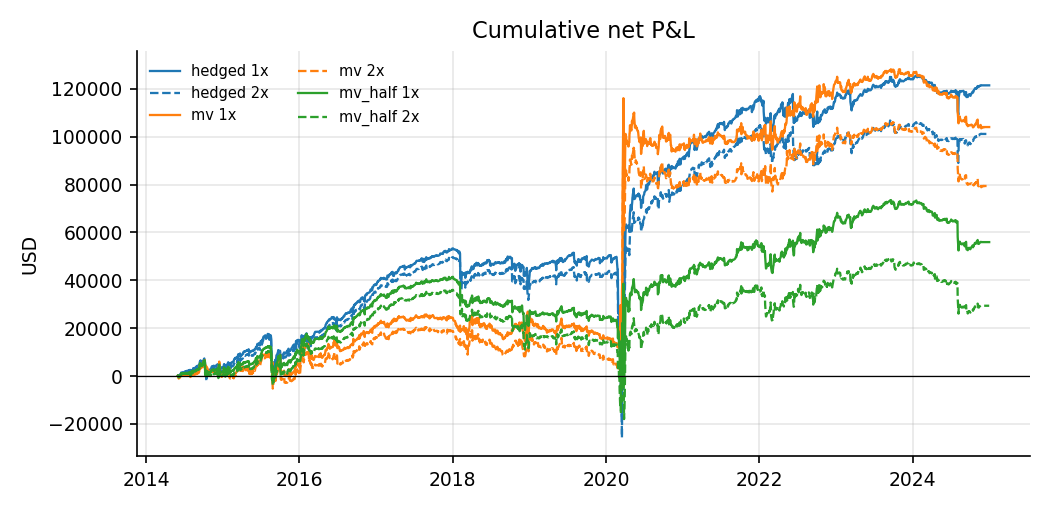
\includegraphics[width=0.92\linewidth]{figures/cum_pnl.png}\caption{Cumulative net P\&L, 1x solid and 2x dashed}\end{figure}

\texttt{mv} trails the reference from 2014 to early 2020, jumps above it in March 2020, falls below it in 2021, leads again from mid-2022 through 2023, and ends 2024 below it. \texttt{mv\_\allowbreak{}half} sits between the two until early 2020, then trails both.

\begin{figure}[H]\centering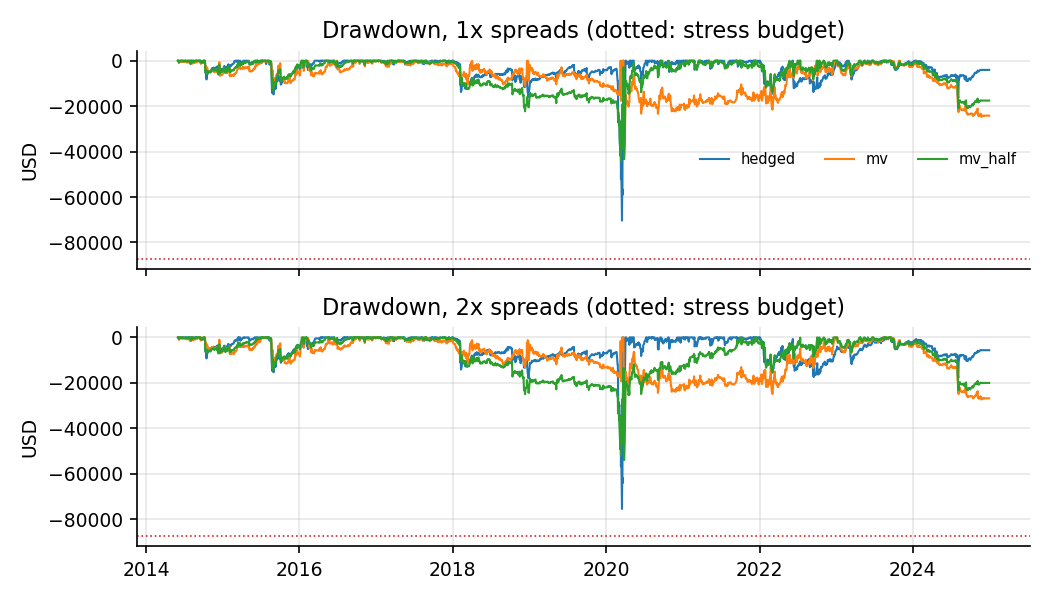
\includegraphics[width=0.92\linewidth]{figures/drawdown.png}\caption{Drawdown at 1x and 2x spreads}\end{figure}

The reference's maximum drawdown runs from January 2018 to 17 March 2020. \texttt{mv}'s is a three-day fall from its 24 March 2020 peak to 27 March 2020, after a large gain. It then stayed below that peak, by up to \$23k (September 2020), until July 2022.

\begin{figure}[H]\centering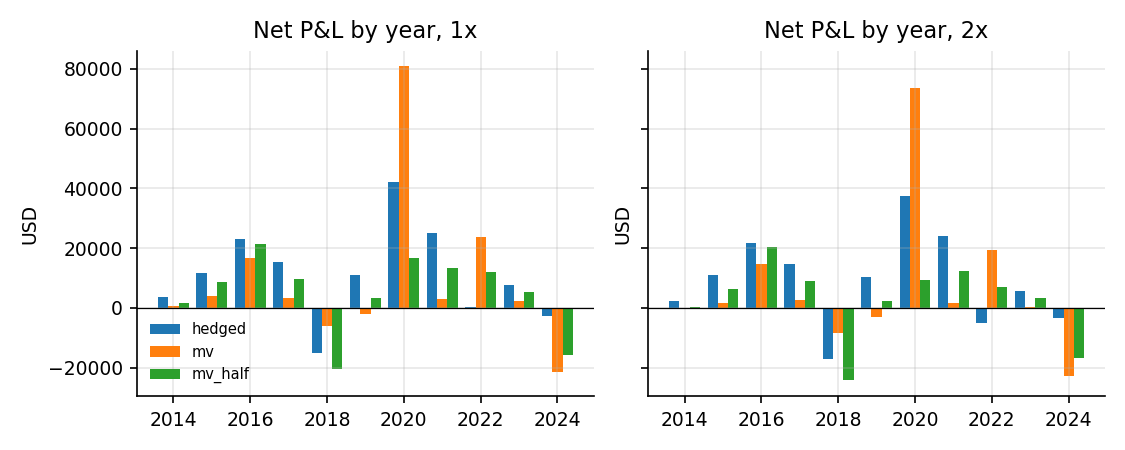
\includegraphics[width=0.92\linewidth]{figures/yearly.png}\caption{Net P\&L by year}\end{figure}

\texttt{mv} made more than the reference in only three years, 2018, 2020 and 2022, all years in which SPY fell for long stretches. It made less in the other eight, most in 2021 (\ensuremath{-}\$22.1k) and 2024 (\ensuremath{-}\$18.8k) at 1x.

\begin{figure}[H]\centering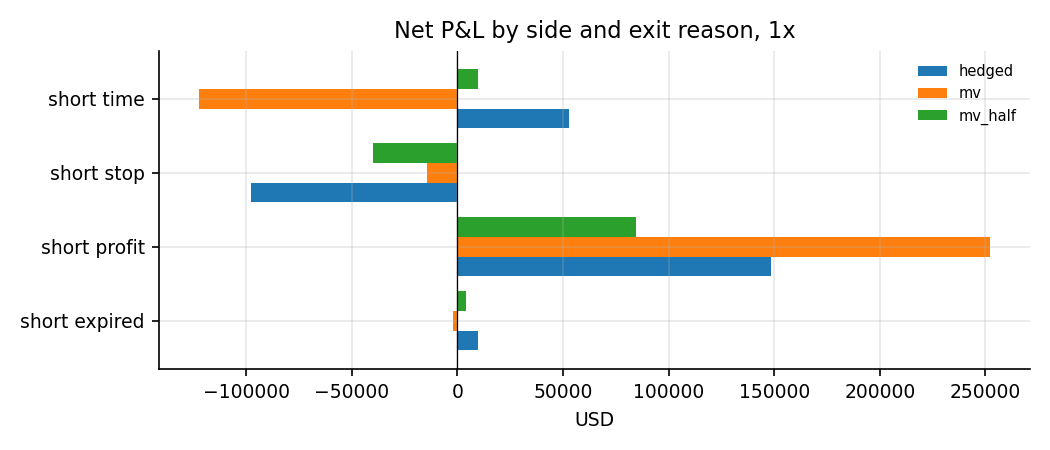
\includegraphics[width=0.92\linewidth]{figures/by_reason.png}\caption{Net P\&L by side and exit reason, 1x}\end{figure}

This chart shows the mechanism. \texttt{mv}'s profit-takes made \$252.3k (42 exits) against \$148.3k (25) for the reference, and its stops lost \$14.4k (4) against \$97.9k (8). Its puts that ran to the 7-DTE time exit lost \$122.4k, against +\$52.9k for the reference.

\begin{figure}[H]\centering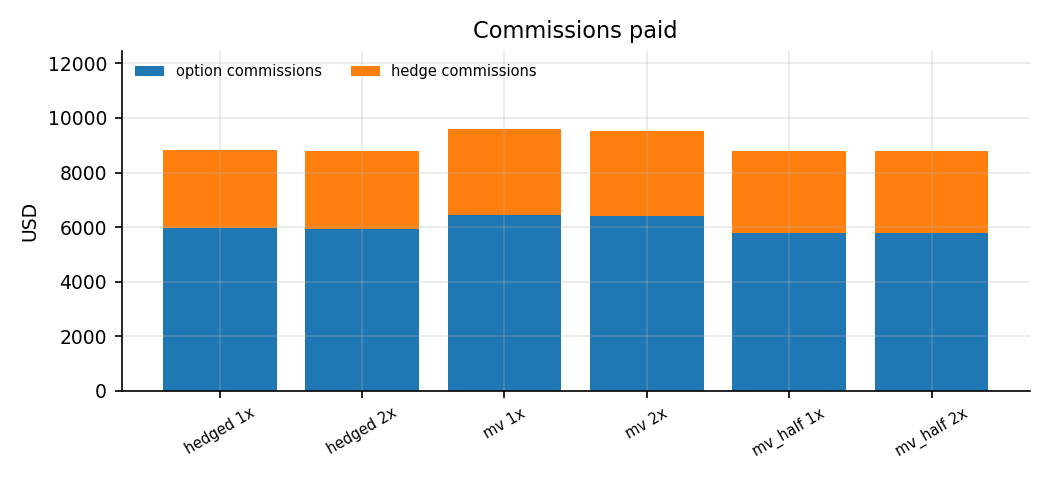
\includegraphics[width=0.92\linewidth]{figures/fees.png}\caption{Commissions paid}\end{figure}

The larger hedge costs little in commissions: \$3,138 against \$2,868 in hedge commissions at 1x, over 2,353 hedge orders against 2,317.

\begin{figure}[H]\centering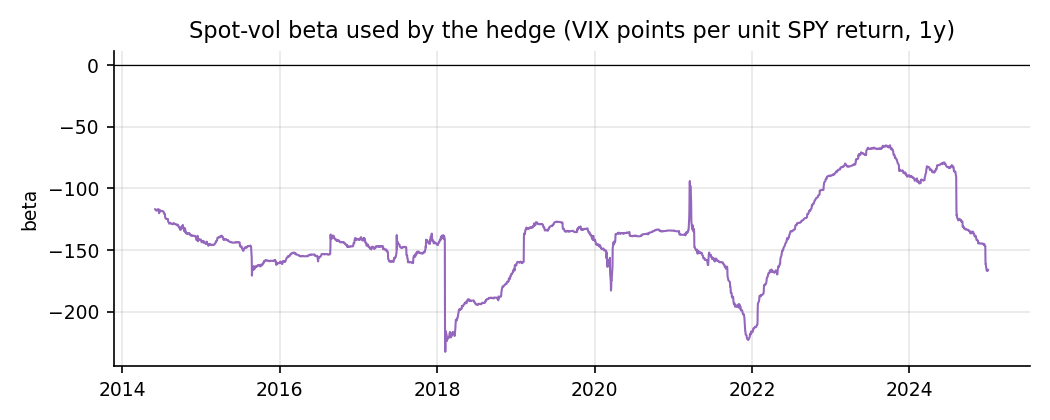
\includegraphics[width=0.92\linewidth]{figures/beta.png}\caption{Spot-vol beta used by the hedge}\end{figure}

\ensuremath{\beta} ranged from \ensuremath{-}232 to \ensuremath{-}65 VIX points per unit SPY return, median \ensuremath{-}142: a 1\% fall in SPY went with about 1.4 VIX points up. It was most negative after February 2018 and from late 2021 to early 2022, and least negative in 2023.

\begin{figure}[H]\centering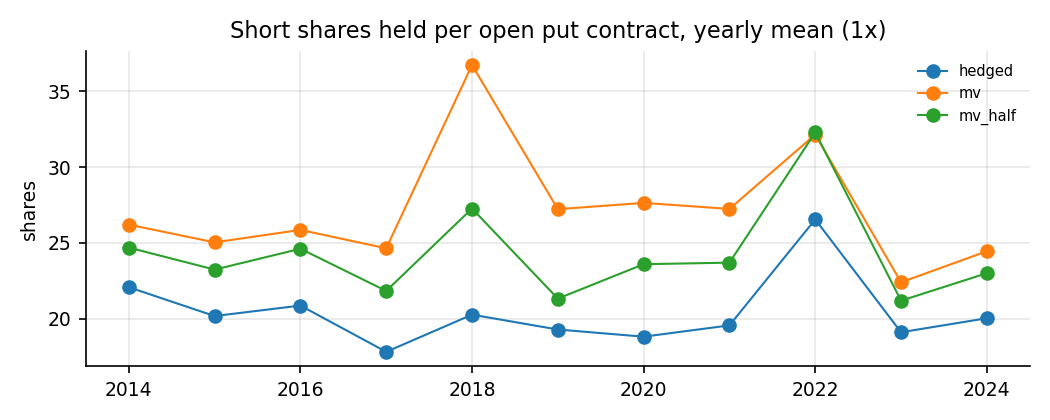
\includegraphics[width=0.92\linewidth]{figures/shares.png}\caption{Short shares per open put contract}\end{figure}

The vega term added about 3-16 short shares per contract to the reference's 18-27 (yearly means at 1x), most in 2018, when \ensuremath{\beta} was most negative.

\begin{figure}[H]\centering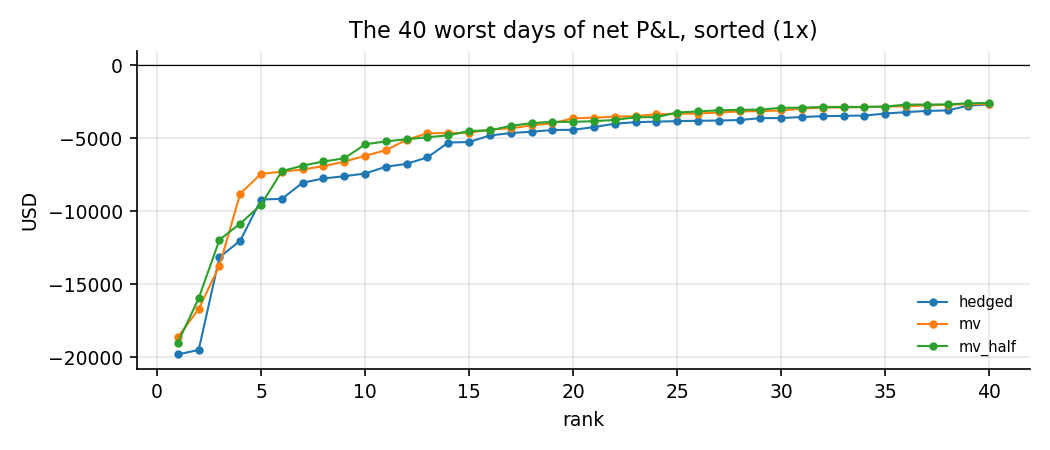
\includegraphics[width=0.92\linewidth]{figures/tail.png}\caption{The 40 worst days of net P\&L}\end{figure}

\texttt{mv}'s worst days are mostly smaller (ranks 1-2 and 4-12; rank 3 is slightly worse). The worst day was \ensuremath{-}\$18.6k against \ensuremath{-}\$19.8k, and the 20 worst days summed to \ensuremath{-}\$144.7k against \ensuremath{-}\$167.0k at 1x.

\section{Analysis}

\textbf{The extra shares are a short SPY position, and the exit rules turn that into an asymmetry.} The stop and the profit-take measure each put's P\&L including its hedge. With more short shares, a fall in SPY lifts the position's P\&L, so puts hit the 50\% profit-take more often (42 against 25) and the stop less often (4 against 8). In a rise the extra shares lose, the put doesn't reach the profit-take, and it is held to the 7-DTE exit. Time exits went from +\$52.9k to \ensuremath{-}\$122.4k. SPY rose over most of 2014-2024, so the extra short exposure cost money in eight of eleven years. This part is mechanical, not noise.

\textbf{March 2020 decides the tail and drawdown checks.} From 19 February to 30 April 2020, \texttt{mv} made \$89.4k at 1x against \$21.7k for the reference; outside that window it made \$14.7k against \$99.8k. In that window \texttt{mv} was never stopped: its 55- and 120-contract puts closed at the profit-take, while the reference was stopped three times before its 100-contract entry. Only 97 of \texttt{mv}'s 193 round trips opened at the same time as one of the reference's (72 with the same close). The paths separate early, so the March 2020 gain comes from one path through one crash.

\textbf{The hedge didn't lower variance.} \texttt{mv}'s daily P\&L standard deviation was higher than the reference's (\$1,515 against \$1,446 at 1x; \$892 against \$776 outside the February-April 2020 window). \texttt{mv\_\allowbreak{}half} had the lowest (\$1,205), but it made the least (\$56.0k), because its March 2020 path was worse: it was stopped on its first put and held the next three to the time exit, making \$11.1k in the window. A result that isn't monotone in k is a sign that path dependence, not the hedge ratio, drives the totals. The lower tail is consistent with Hull \& White's idea that the put's hidden long-SPY exposure matters in falls. But on this book the price of that protection, paid in every rising year, was larger than the P\&L allowance.

\section{Verdict}

Failed, per the pre-registered bar: the tail and drawdown checks passed at 1x and 2x, but net P\&L was \$12.4k (1x) and \$16.7k (2x) further below the reference than the \$5k allowed. Archive this card.

A follow-up would need its own card, and should separate the hedge from the exit rules. One option is to measure the stop and the profit-take on the option alone, so the hedge only changes risk. Another is a \ensuremath{\beta} fitted on the put's own IV rather than VIX.

\section{Caveats}

\begin{itemize}

\item \textbf{In-sample:} the idea comes from the 2026-09-27 leverage-effect report. The book was chosen after its 2014-2024 results. Before pre-registration, the card's reporting code was tested on the reference run and the features file, which showed the median \ensuremath{\beta}.

\item \textbf{One crash decides the tail result:} most of \texttt{mv}'s lower drawdown and higher 2020-24 P\&L comes from one path through February-April 2020.

\item \textbf{Approximations in the hedge:}

\begin{itemize}

\item VIX stands in for the change in the put's own IV.

\item \ensuremath{\beta} is a walk-forward VIX regression, not Hull \& White's fitted coefficients.

\item The stress sizing ignores the extra shares.

\end{itemize}

\item \textbf{Spread model:} fitted on about two weeks of calm 2026 live quotes. Fills of up to 120 contracts use the one-contract model; the 2x run is the stress test.

\item \textbf{Data gaps:} R2 has no month-end weekdays, so about 3.3\% of scheduled times are skipped; 15 hedge times had no delta.

\item \textbf{Margin:} not modelled.

\end{itemize}

\section{Trials}

4 trials for this experiment (2 variants \ensuremath{\times} 1x and 2x, one run of \texttt{experiment.\allowbreak{}py}). The \texttt{hedged} reference and the baseline were reused, not rerun.

The registry tags the \texttt{mv} 1x row 79b09a1-dirty and the other three 3568520-dirty. Other cards of the same batch were pre-registered, and had uncommitted files in the shared working tree, while this run was going. The engine, \texttt{configs/\allowbreak{}backtest.\allowbreak{}toml} and this card's config, card and script are unchanged between the pre-registration commit 3ab834b and both tags.

The pass bar was not changed.

\end{document}
